% =========================
% Figure: egpMC_deviations (normalized terms entering D)
% =========================
% Preamble needs:
% \usepackage{pgfplots}
% \pgfplotsset{compat=1.18}
\begin{figure}[htbp]
\centering
\begin{tikzpicture}
\begin{axis}[
    ybar,
    width=\textwidth,
    height=7cm,
    ymin=0,
    bar width=8pt,
    enlarge x limits=0.08,
    xlabel={Criterion (normalized term in $D$)},
    ylabel={Weighted deviation},
    xtick=data,
    xticklabel style={rotate=45, anchor=east},
    xticklabels={
      Height $(\tfrac{1}{47}n_1)$,
      Capacity $(\tfrac{1}{3}n_2)$,
      Res.~area $(\tfrac{1}{0.04}p_3)$,
      Temp $(\tfrac{1}{0.04}p_4)$,
      Pop. $(\tfrac{1}{48.74}n_5)$,
      Rain $(\tfrac{1}{0.52}n_6)$,
      Residence $(\tfrac{1}{22.07}p_7)$,
      Farm dist. $(\tfrac{1}{0.32}p_8)$,
      Nearest road $(\tfrac{1}{0.23}p_9)$,
      Farm area $(\tfrac{1}{0.68}n_{10})$
    },
    nodes near coords,
    nodes near coords align={vertical},
    every node near coord/.append style={font=\scriptsize, /pgf/number format/precision=4, /pgf/number format/fixed},
    grid=both,
    grid style={opacity=0.2},
    legend style={at={(0.02,0.98)},anchor=north west,draw=none,fill=none}
]
% Normalized deviations entering D:
% n1=0, n2=0, p3/0.04=10.5, p4/0.04=0, n5=0, n6=0, p7/22.07≈0.6203, p8/0.32=12.3438, p9/0.23=25.1304, n10=0
\addplot coordinates {
 (1,0.0000) (2,0.0000) (3,10.5000) (4,0.0000) (5,0.0000)
 (6,0.0000) (7,0.6203) (8,12.3438) (9,25.1304) (10,0.0000)
};
% Draw D* as a reference line
\addplot+[domain=0.5:10.5, samples=2] {25.1304};
\addlegendentry{$D^{\star}=25.1304$}
\end{axis}
\end{tikzpicture}
\caption{EGP--MCGP normalized deviations in the minimax term $D$. The binding criterion is \emph{Nearest road} with $p_9/0.23=D^{\star}$; next are Farmland distance and Reservoir area.}
\label{fig:egpMCGPDeviations}
\end{figure}